\documentclass[../main.tex]{subfiles}

\begin{document}
\section{Procedure} \label{sec:procedure}
\subsection{Calibration} \label{sec:calibration-procedure}
The monocular co-registration procedure introduced in section~\ref{sec:monocular-coregistration} can be extended and formalised as a novel non-metric calibration procedure suitable for our camera array. The key part of the procedure lies in the estimation of geometric transforms that relate image pairs captured by the camera array, relative to some reference plane. To achieve this, we can capture a full array image of a calibration pattern positioned at the reference plane. This image set will be called the \emph{calibration set}, and it will inform our estimation. 

\subsubsection{Capturing an effective calibration set}
Our first step is to choose an appropriate reference plane at which to situate the calibration pattern. The reference plane should be one that provides sufficient overlap across camera views, so that common features can be matched (see figure~\ref{fig:overlap}).

\begin{figure}[H]
    \centering
    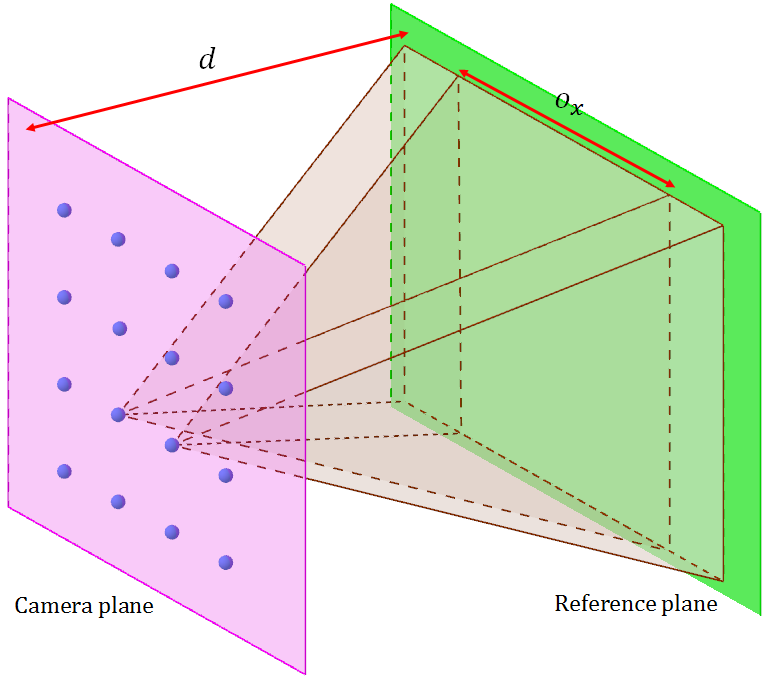
\includegraphics[width=0.6\linewidth]{images/overlap}
    \caption{Diagram of our camera array and reference plane. Two camera views are projected onto the reference plane, which is set up at distance $d$ from the camera plane. Significant overlap in the $x$ direction is illustrated as $o_x$. }
    \label{fig:overlap}
\end{figure}

\newpage
It is clear that the degree of overlap between any two camera images is a function of each camera's pose, field of view, translation, as well as the distance $d$ from each camera to the reference plane. For a coplanar setup with uniform viewing directions, overlap increases logarithmically with $d$. Thus we should consider that as $d$ increases for such setups, so does the required size of the calibration pattern. Additionally, if we consider the camera array a virtual camera, then the ratio between the synthetic aperture size and our synthetic focal length (this focal length is also given by $d$) will have a significant effect on the focal sensitivity of light fields. Clearly, the most practical calibration setup will depend on the resources available, the camera setup, and the intended use of the camera. For our calibration setup, see section~\ref{sec:calibration-implementation}.

After choosing an appropriate reference plane, we can choose a calibration pattern. Most calibration procedures involve a checkerboard pattern, but this is inappropriate for our procedure since we rely on the detection of \emph{unique} features across images. Checkerboards and other repeating patterns have non-unique surface features which can easily be mismatched with other identical features. Therefore, the calibration pattern must be sufficiently detailed and non-repeating. The colourful impressionistic paintings of Leonid Afremov have proven effective for our setup.

Once we have a calibration set that meets the aforementioned requirements, we can begin to develop our transformation set for rectification. 

\subsubsection{Calculating the geometric transforms between reference plane views}
For each image in the calibration set, we can identify surface features automatically via the Speeded Up Robust Feature detection algorithm (SURF) \cite{bay2006surf}. SURF has been shown to identify sufficient features quickly and effectively. We can then identify unique matching surface features between successive image pairs, and thus estimate their relative geometric transforms. Estimating geometric transforms can be achieved by applying a \emph{RANdom SAmple Consensus} algorithm (RANSAC). We have opted to use \emph{M-estimator SAmple and Consensus} (MSAC), which additionally evaluates the quality and likelihood of the consensus set \cite{torr2000mlesac}. We can exploit this to enforce a minimum confidence level required to produce a positive match. A MATLAB implementation of our calibration procedure is provided in appendix \ref{apx:matlab-build-transforms}.

\subsubsection{Measuring calibration accuracy} \label{sec:assessing-calibration}
To quickly assess the accuracy of our transformation set, we can use the transformation set to project all the images from the \emph{calibration set} onto a new image plane, effectively constructing a panorama. It turns out that constructing such a panorama provides an effective means to visually assess the quality of the transformation set (see figure~\ref{fig:panoramas}). A good transformation set will result in a smoothly stitched panorama. 

\begin{figure}[H]
    \centering
    
\includegraphics[width=\linewidth]{images/panoramas}
    \caption{Jagged panorama of a calibration set (left) and smooth panorama of a calibration set (right). The calibration set used to construct the smooth panorama will produce better results for light field applications. The jagged panorama was built using a poor calibration set which was not of a fully planar scene. Ignore any clear differences in colour across the panoramas - this is due to automatic colour balancing and gamma correction in the camera modules.}
    \label{fig:panoramas}
\end{figure}

To more accurately assess the quality of a transformation set, we can evaluate the positional consistency of surface features across images in the panorama, one image at a time. The closer each surface feature is to having a uniform position across images, the better the transformation set is for light field applications.

\newpage
\subsection{Rectification} \label{sec:rectification}
A transformation set built using the procedure described in the previous section (section~\ref{sec:calibration-procedure}) can be used to rectify any set of images captured by the camera array. Rectification will bring images into light field alignment and enable popular light field applications such as synthetic aperture focusing.

In section~\ref{sec:assessing-calibration}, we suggested that projecting calibration images onto plane (effectively constructing a panorama) is useful as a quick way to assess the accuracy of a transformation set. This is very similar to the rectification process. To rectify an image, we can simply project only the image of interest onto the 'panorama plane' using the appropriate transformation (see figure~\ref{fig:rectification}). Repeating this for all images in a set will rectify the set for light field acquisition and rendering. This effectively brings all images into alignment so that when rendered as a light field, the focus is on the reference plane. Focus can then be easily adjusted to any other parallel plane. A MATLAB implementation of the rectification procedure is provided in appendix \ref{apx:matlab-rectify-images}.

\begin{figure}[H]
    \centering
    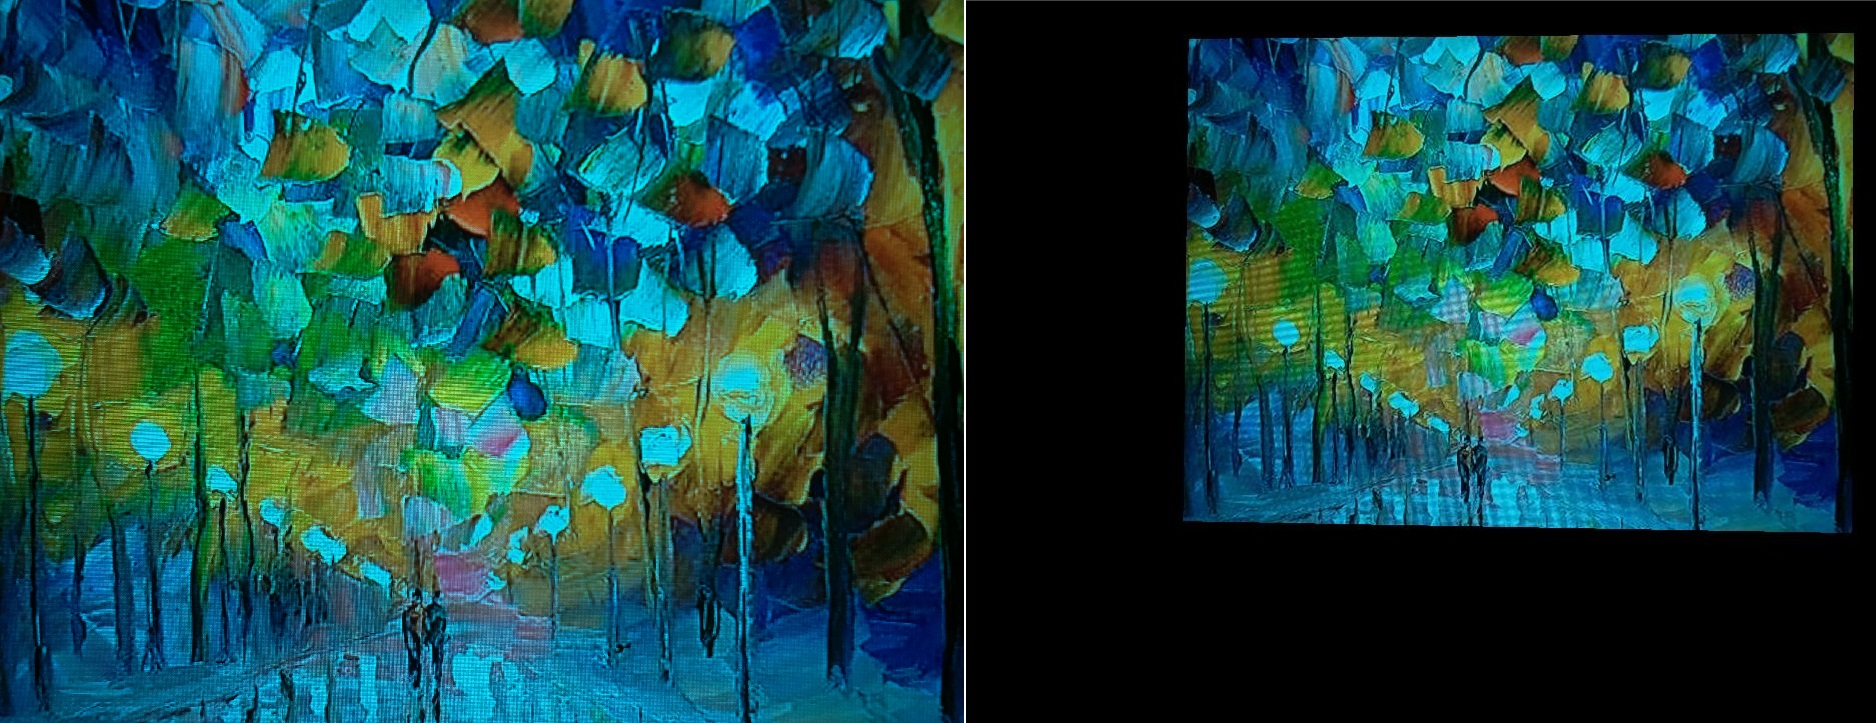
\includegraphics[width=\linewidth]{images/rectification}
    \caption{Original image (left) and rectified image (right).}
    \label{fig:rectification}
\end{figure}

\newpage
Rectified images have a side effect of having potentially large areas of blackness. This may be inconvenient or significantly affect the file size of large sets. It is possible to crop rectified images, but this also requires that the relative positions of cameras be known. This is because the translations between cropped portions must correspond to the relative camera positions associated with each image. Cropped images must also be of uniform dimensions. We illustrate both possibilities (see figure~\ref{fig:cropped-vs-uncropped}).

\begin{figure}[H]
    \centering
    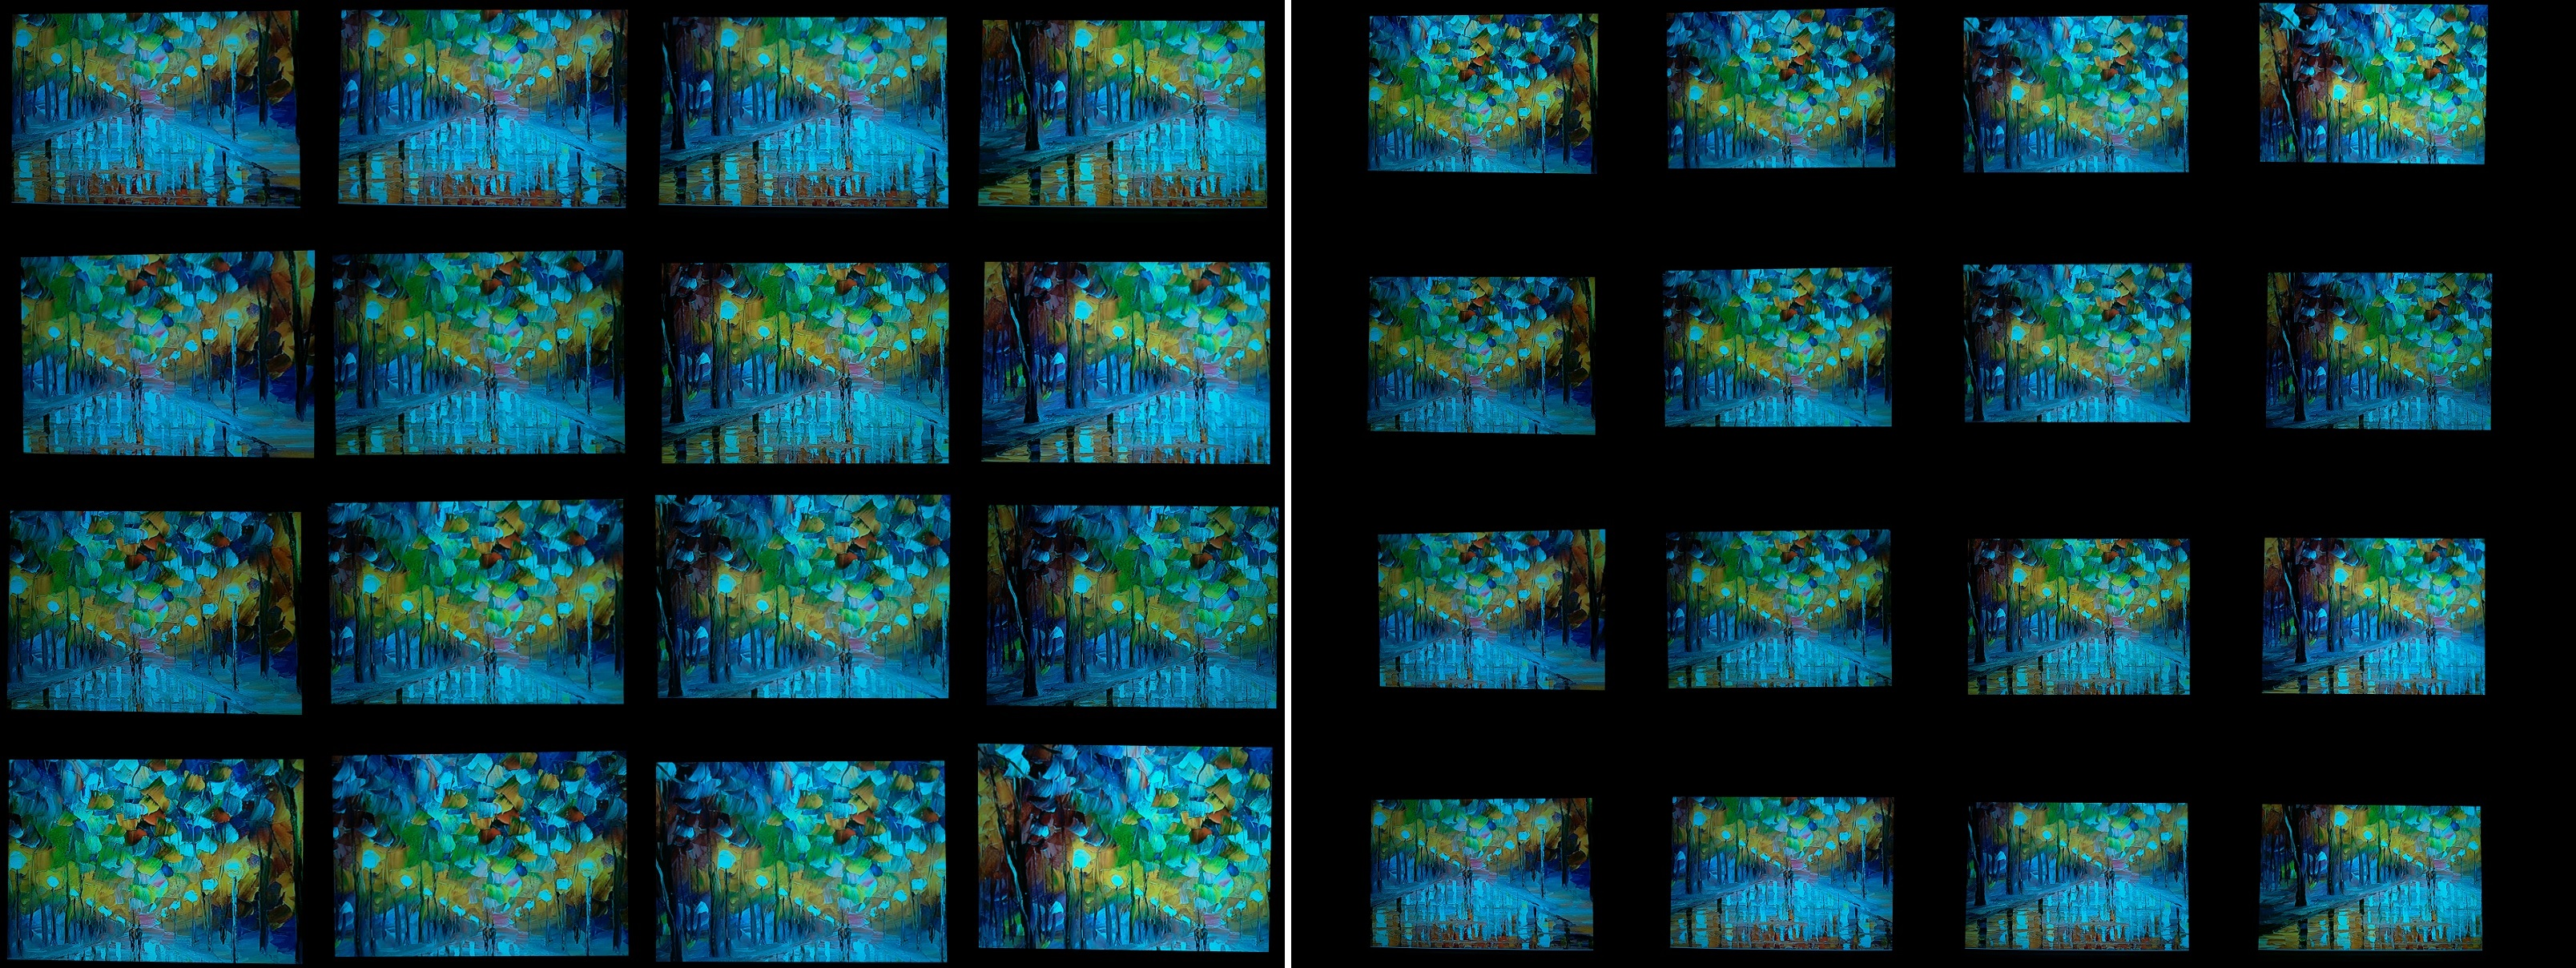
\includegraphics[width=\linewidth]{images/cropped-vs-uncropped}
    \caption{Cropped set (left) vs. uncropped set (right). In the uncropped set, each image is the size of a full panorama.}
    \label{fig:cropped-vs-uncropped}
\end{figure}

\newpage
\end{document}